The architecture revolves primarily around the raspberry pi computer itself.  The interface of the raspberry pi will communicate with all other major systems sending commands and receiving data.  The first major system to communicate with is the vision system.  This system is responsible for the cameras and has two that are part of it: the IR camera, and the 3D camera.  Both will connect to the PI's interface in order to transmit visual data.  This data will be redirected by the interface to the Pre-processing unit which will determine what raw film data is worth keeping and what is not by a factor of cars in the streets.  Data kept is placed into storage which the interface can then pull out again.  It is powered by a socket connected to the power system, an outlet inside the users home.  The case system has a cooling unit which prevents the PI from overheating through a ventilation shaft.  This fan draws power from the PI via its interface.  When the PI is connected to the user's computer via Ethernet, it will automatically run its application on their computer.  This application receives transferred data from the PI's storage and processes it, splitting meta data into a database and film data into local storage.  All of this data will be accessible to the user via a graphic user interface.

\begin{figure}[h!]
	\centering
 	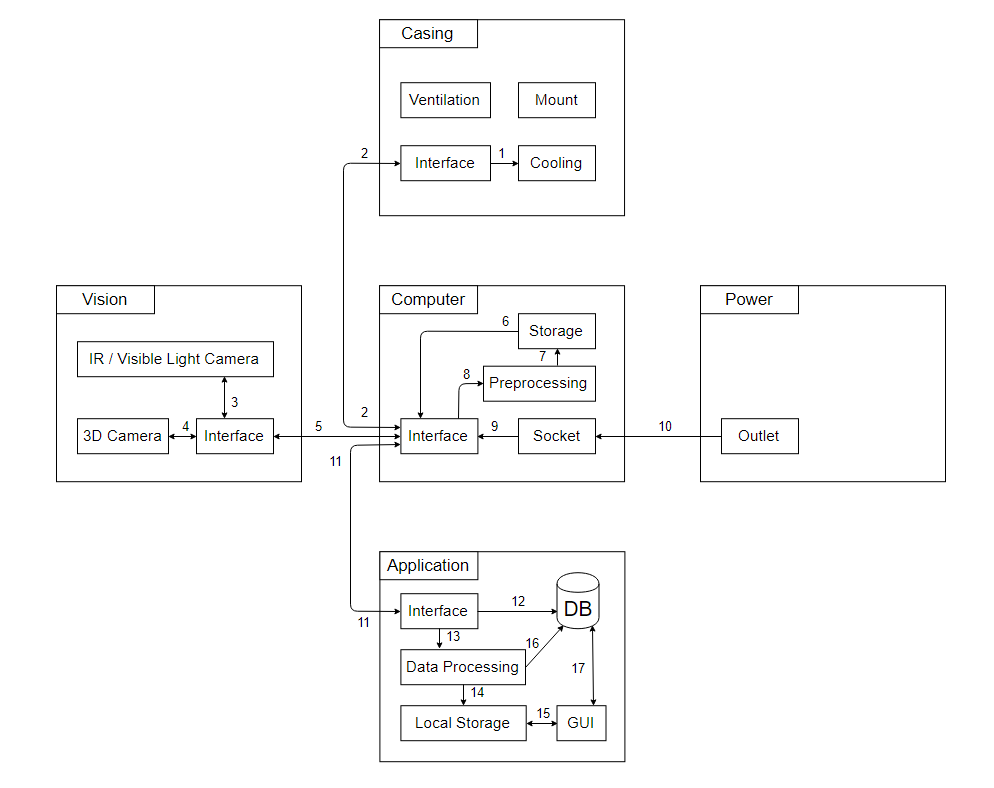
\includegraphics[width=0.60\textwidth]{images/ADS.png}
 \caption{A simple architectural layer diagram}
\end{figure}

\subsection{Layer Computer Description}
The main purpose of the computer layer is to the central source of communication and serve as the collector and organizer of data received from the vision layer. Maintaining power granted by the power layer and distribute to the cooling system, cameras, and itself to function as desired. Allowing to request proper cooling from the case layer to maintain functionality of the Traffic Pi without worrying about unstable temperature both generated from internal and environmental. The computer layer will take in raw data from the vision layer, such as footage (frames), distance, and lighting, after detecting cars passing by. Pre-processing will take in effect, time stamping frames and formatting data, then direct to the storage for later use by the application layer.

\subsection{Layer Vision Description}
The vision layer comprises of the physical cameras, IR / visible light and 3D cameras, that views the road and transmit the footage data to the Traffic Pi's pre-processing and stored for later. The IR / visible light camera would be able to view the road and passing vehicles in both day and night settings. The 3D camera will be able to measure the distance of the passing vehicles from the camera in every passing frames. While collecting data, until function completion is met, the footage / frames and distance will to send to the computer layer.

\subsection{Layer Application Description}
The main purpose of the application layer is to handle the actual processing of the raw video on the users local machine coming from the computer layer. During the video processing, bounding boxes will be placed around every appropriate vehicle and speed will be measured and recorded. The resulting data will be stored on a local database. Meanwhile, the resulting video will be stored on the users local storage. This layer provides the user with a graphical user interface in order to interact with the system. Using the GUI, the user will be able to view the analyzed video and will have the option be presented with a dashboard fitted with the visual representation of the analytics regarding the traffic study. The user will also have the option of a quick guide and options to download the file of data.

\subsection{Layer Case Description}
The case layer is designed to house every component in a self contained physical structure. The case is designed such that the heat generated from the Raspberry Pi, IR camera, and 3D camera will be able to dissipate quickly away from the system. This ventilation works in conjunction with the cooling subsystem. The cooling component is a small fan that will be attached to the case layer and provide additional temperature control to the Traffic Pi system as a whole. Both the ventilation and cooling component of the case layer are designed to minimize the effects of heat generation on the system. Although the ventilation subsystem is simply a built-in designed component of the case, it is referred to as its own subsystem as it has its own unique functionality. The case layer also includes a mounting plate subsystem which is a physical component designed to make mounting of the Traffic Pi system on a tripod or other auxiliary surface easier. Finally, a USB Type C cable called the interface is the last subsystem designated as part of the case layer. This component is responsible for running power from the Raspberry Pi to the cooling fan subsystem.

\subsection{Layer Power Description}
The power layer is specified for explicit visualization of the providing power to the system. This layer consists of only one subsystem, the outlet. Outlet is defined as any US AC power outlet providing 120V at 60Hz. A power cable is run from this outlet to the Raspberry Pi to provide power to it and by extension each of the other layers. 